\documentclass[letterpaper, 12pt]{article}
\usepackage[utf8]{inputenc}
\usepackage[top=2.54cm,right=2cm,left=2cm,bottom=2.54cm]{geometry}
% \usepackage{helvet}
% \renewcommand{\familydefault}{\sfdefault}
\usepackage{float,amssymb,tabu,booktabs,multirow,multicol,subfig,graphicx,tikz,pgfplots,amsmath,mathtools,subfigure,subcaption}
\usepackage{listings}
\usepackage[shortlabels]{enumitem}
\definecolor{codegreen}{rgb}{0,0.6,0}
\definecolor{codegray}{rgb}{0.5,0.5,0.5}
\definecolor{codepurple}{rgb}{0.58,0,0.82}
\definecolor{backcolour}{rgb}{0.95,0.95,0.92}
% \onehalfspacing
\lstdefinestyle{mystyle}{
    backgroundcolor=\color{backcolour},   
    commentstyle=\color{codegreen},
    keywordstyle=\color{magenta},
    numberstyle=\tiny\color{codegray},
    stringstyle=\color{codepurple},
    basicstyle=\footnotesize,
    breakatwhitespace=false,         
    breaklines=true,                 
    captionpos=b,                    
    keepspaces=true,                 
    numbers=left,                    
    numbersep=5pt,                  
    showspaces=false,                
    showstringspaces=false,
    showtabs=false,                  
    tabsize=2
}
 
\lstset{style=mystyle}
 
\usepackage{amsmath}
\usepackage[numbers]{natbib}
\usepackage{hyperref}
\hypersetup{
    colorlinks=true,
    linkcolor=black,
    citecolor=cyan,
    filecolor=blue,
    urlcolor=magenta,
}
\usepackage{fancyhdr}
\pagestyle{fancy}
\fancyhf{}
\fancyhead[LE,RO]{Dalton Daniel, Guanyun Liu}
\fancyhead[RE,LO]{Nonlinear Final Project}
\fancyhead[CE,CO]{}
\fancyfoot[CE,CO]{\thepage}

\title{Nonlinear Final project}
\author{Dalton Daniel, Guanyun Liu}
\date{May 2022}

\begin{document}
\maketitle
\section{Motivation}
Given that self driving cars want to achieve more general use it is important that they are able to achieve the final stage of the driving process, parking. To do this they need to navigate through the various obstacles of a parking lot into a desired space and make sure not to hit adjacent cars. Additionally the final state needs to be within a certain region so the user can get out of the car without hitting the cars next to them with their doors.To add further complications manufacturing specifications may allow a certain degree of error to the car resulting in some amount of uncertainty in the controls. From all of this a robust controller is needed to achieve the desired results.
\section{Problem Setup}
The chosen controller will be a rear-wheel drive car, with some simplifications for use with DDP trajectory generation. One major simplification will be that the length between axles is treated as 1m. To accommodate this the car's overall size will be treated as 1.66m long and .66m wide, to attempt to mimic actual car size ratios (originally approximated as 2m$\times$5m with 3m wheelbase). The car will navigate through a parking lot and come to a complete stop in a parking-space. The car's controls are acceleration with a multiplicative uncertainty based on a 5\% tolerance, and steering wheel turning $\dot{\phi}$ with a constant $3.3^\circ$ uncertainty. To accommodate the DDP method and car dimensions obstacles will be treated as 1m larger in radius (larger will be shown on graph). To accommodate the controller the system will also be considered to be starting with some velocity.
\section{Control Derivation}
Given the dynamics of a rear-wheel-drive car-like model,
\begin{flalign}
  \dot{x} & = v\text{cos}(\theta)\nonumber\\
  \dot{y} & = v\text{sin}(\theta)\nonumber\\
  \dot{\theta} & = \frac{v\text{tan}(\phi)}{l}\\
  \dot{v} & = u_1\nonumber\\
  \dot{\phi} & = u_2\nonumber
\end{flalign}
Choose the flat output $Y = (x,~y)^T$, and then keep differentiating the outputs until inputs appears with a linear relationship.
\begin{flalign}
  \ddot{Y}_1 & = \ddot{x} = u_1 \text{cos}(\theta) - v^2\text{sin}(\theta)\text{tan}(\phi)\nonumber\\
  & \\
  \ddot{Y}_2 & = \ddot{y} = u_1\text{sin}(\theta) + v^2\text{cos}(\theta)\text{tan}(\phi)\nonumber
\end{flalign}
The second order differentiation of the flat outputs only contains $u_1$. Hence, we need to differentiate it further to get the second input.
\begin{flalign}\label{eq:3rd-order-eqns}
  Y^{(3)}_1 & = x^{(3)} = -3u_1v\text{sin}(\theta)\text{tan}(\phi) - v^3\text{cos}(\theta)\text{tan}^2(\phi) + \dot{u}_1\text{cos}(\theta)-v^2\text{sin}(\theta)\text{sec}^2(\phi)u_2\nonumber\\
  & \\
  Y^{(3)}_2 & = y^{(3)} = 3u_1v\text{cos}(\theta)\text{tan}(\phi) - v^3\text{sin}(\theta)\text{tan}^2(\phi) + \dot{u}_1\text{sin}(\theta)+v^2\text{cos}(\theta)\text{sec}^2(\phi)u_2\nonumber
\end{flalign}
Rewrite Eq.~\ref{eq:3rd-order-eqns} in the matrix form,
\begin{equation}\label{eq:3rd-order-eqns-matrixForm}
  Y^{(3)} = 
  \begin{bmatrix}
    x^{(3)}\\
    y^{(3)}
  \end{bmatrix}
  =
  \begin{bmatrix}
    -3u_1v\text{sin}(\theta)\text{tan}(\phi) - v^3\text{cos}(\theta)\text{tan}^2(\phi)\\
    3u_1v\text{cos}(\theta)\text{tan}(\phi) - v^3\text{sin}(\theta)\text{tan}^2(\phi)
  \end{bmatrix}
  +
  \begin{bmatrix}
   \text{cos}(\theta) & -v^2\text{sin}(\theta)\text{sec}^2(\phi)\\
    \text{sin}(\theta) & v^2\text{cos}(\theta)\text{sec}^2(\phi)
  \end{bmatrix}
  \begin{bmatrix}
    \dot{u}_1\\
    u_2
  \end{bmatrix}
\end{equation}
In this case, we choose $u = \begin{bmatrix}
  \dot{u}_1\\
  u_2
\end{bmatrix}$ as our controls and set $u_1$ as a dynamic compensator $\xi$. Also, $Y^{(3)}$ is our virtual input $v$, that is $y^{(3)} = v$. As a result, re-arranging Eq .~\ref{eq:3rd-order-eqns-matrixForm} gives us the control law (where $v\neq 0$).
\begin{equation}\label{eq:control-laws}
    \begin{bmatrix}
      \dot{u}_1\\
      u_2
    \end{bmatrix} = 
    \begin{bmatrix}
      \text{cos}(\theta) & \text{sin}(\theta)\\
      \frac{\text{sin}(\theta)(\text{sin}^2(\phi)-1)}{v^2} & \frac{\text{cos}(\theta)\text{cos}^2(\phi)}{v^2} 
    \end{bmatrix}
    \Bigg(v - 
  \begin{bmatrix}
      -3u_1v\text{sin}(\theta)\text{tan}(\phi) - v^3\text{cos}(\theta)\text{tan}^2(\phi)\\
      3u_1v\text{cos}(\theta)\text{tan}(\phi) - v^3\text{sin}(\theta)\text{tan}^2(\phi)
  \end{bmatrix}
  \Bigg)
\end{equation}
To track the desired trajectory,
\begin{equation}\label{eq:virtual-input}
    v = Y^{(3)}_d(t) - K_1 [Y(t) - Y_d(t)] - K_2[\dot{Y}(t) - \dot{Y}_d(t)] - K_3[\ddot{Y}(t) - \ddot{Y}_d(t)]
\end{equation}
In our case, we choose $K_1 = 
\begin{bmatrix}
    2000 & 0\\
    0 & 2000
\end{bmatrix}$,
$K_2 = 
\begin{bmatrix}
    300 & 0 \\ 0 & 300
\end{bmatrix}$
, and $K_3 = 
\begin{bmatrix}
    10 & 0\\ 0 & 10
\end{bmatrix}$.\\

\noindent Define the error state $z\in \mathbb{R}^6$ as
\begin{equation}
    z = 
    \begin{bmatrix}
        Y(t) - Y_d(t)\\
        \dot{Y}(t) - \dot{Y}_d(t)\\
        \ddot{Y}(t) - \ddot{Y}_d(t)
    \end{bmatrix}
\end{equation}
Then, the control laws of Eq.~\ref{eq:control-laws} and \ref{eq:virtual-input} gives the closed-loop linear dynamics as 
\begin{equation}
    \dot{z} = Az
\end{equation}
Where
\begin{equation*}
    A =
    \begin{bmatrix}
        0 & 0 & 1 & 0 & 0 & 0\\
        0 & 0 & 0 & 1 & 0 & 0\\
        0 & 0 & 0 & 0 & 1 & 0\\
        0 & 0 & 0 & 0 & 0 & 1\\
        -2000 & 0 & -300 & 0 & -10 & 0\\
        0 & -2000 & 0 & -300 & 0 & -10\\
    \end{bmatrix}
\end{equation*}
The eigenvalues of A are 
\begin{equation*}
    \lambda = 
    \begin{bmatrix}
    -7.1523 + 0.0000i\\
    -1.4239 +16.6615i\\
    -1.4239 -16.6615i\\
    -1.4239 +16.6615i\\
    -1.4239 -16.6615i\\
    -7.1523 + 0.0000i\\
    \end{bmatrix}
\end{equation*}
Since all eigenvalues have negative real parts, the closed-loop linear dynamics is asymptotically stable. It means theoretically, our control can track the desired trajectory.
\section{Results}
It should be noted that due to issues with DDP the final position was not reached however, the tracker followed the desired trajectory well meaning that if a trajectory which achieves the desired goal is made the control law should be able to follow it.
\begin{figure}
    \centering
    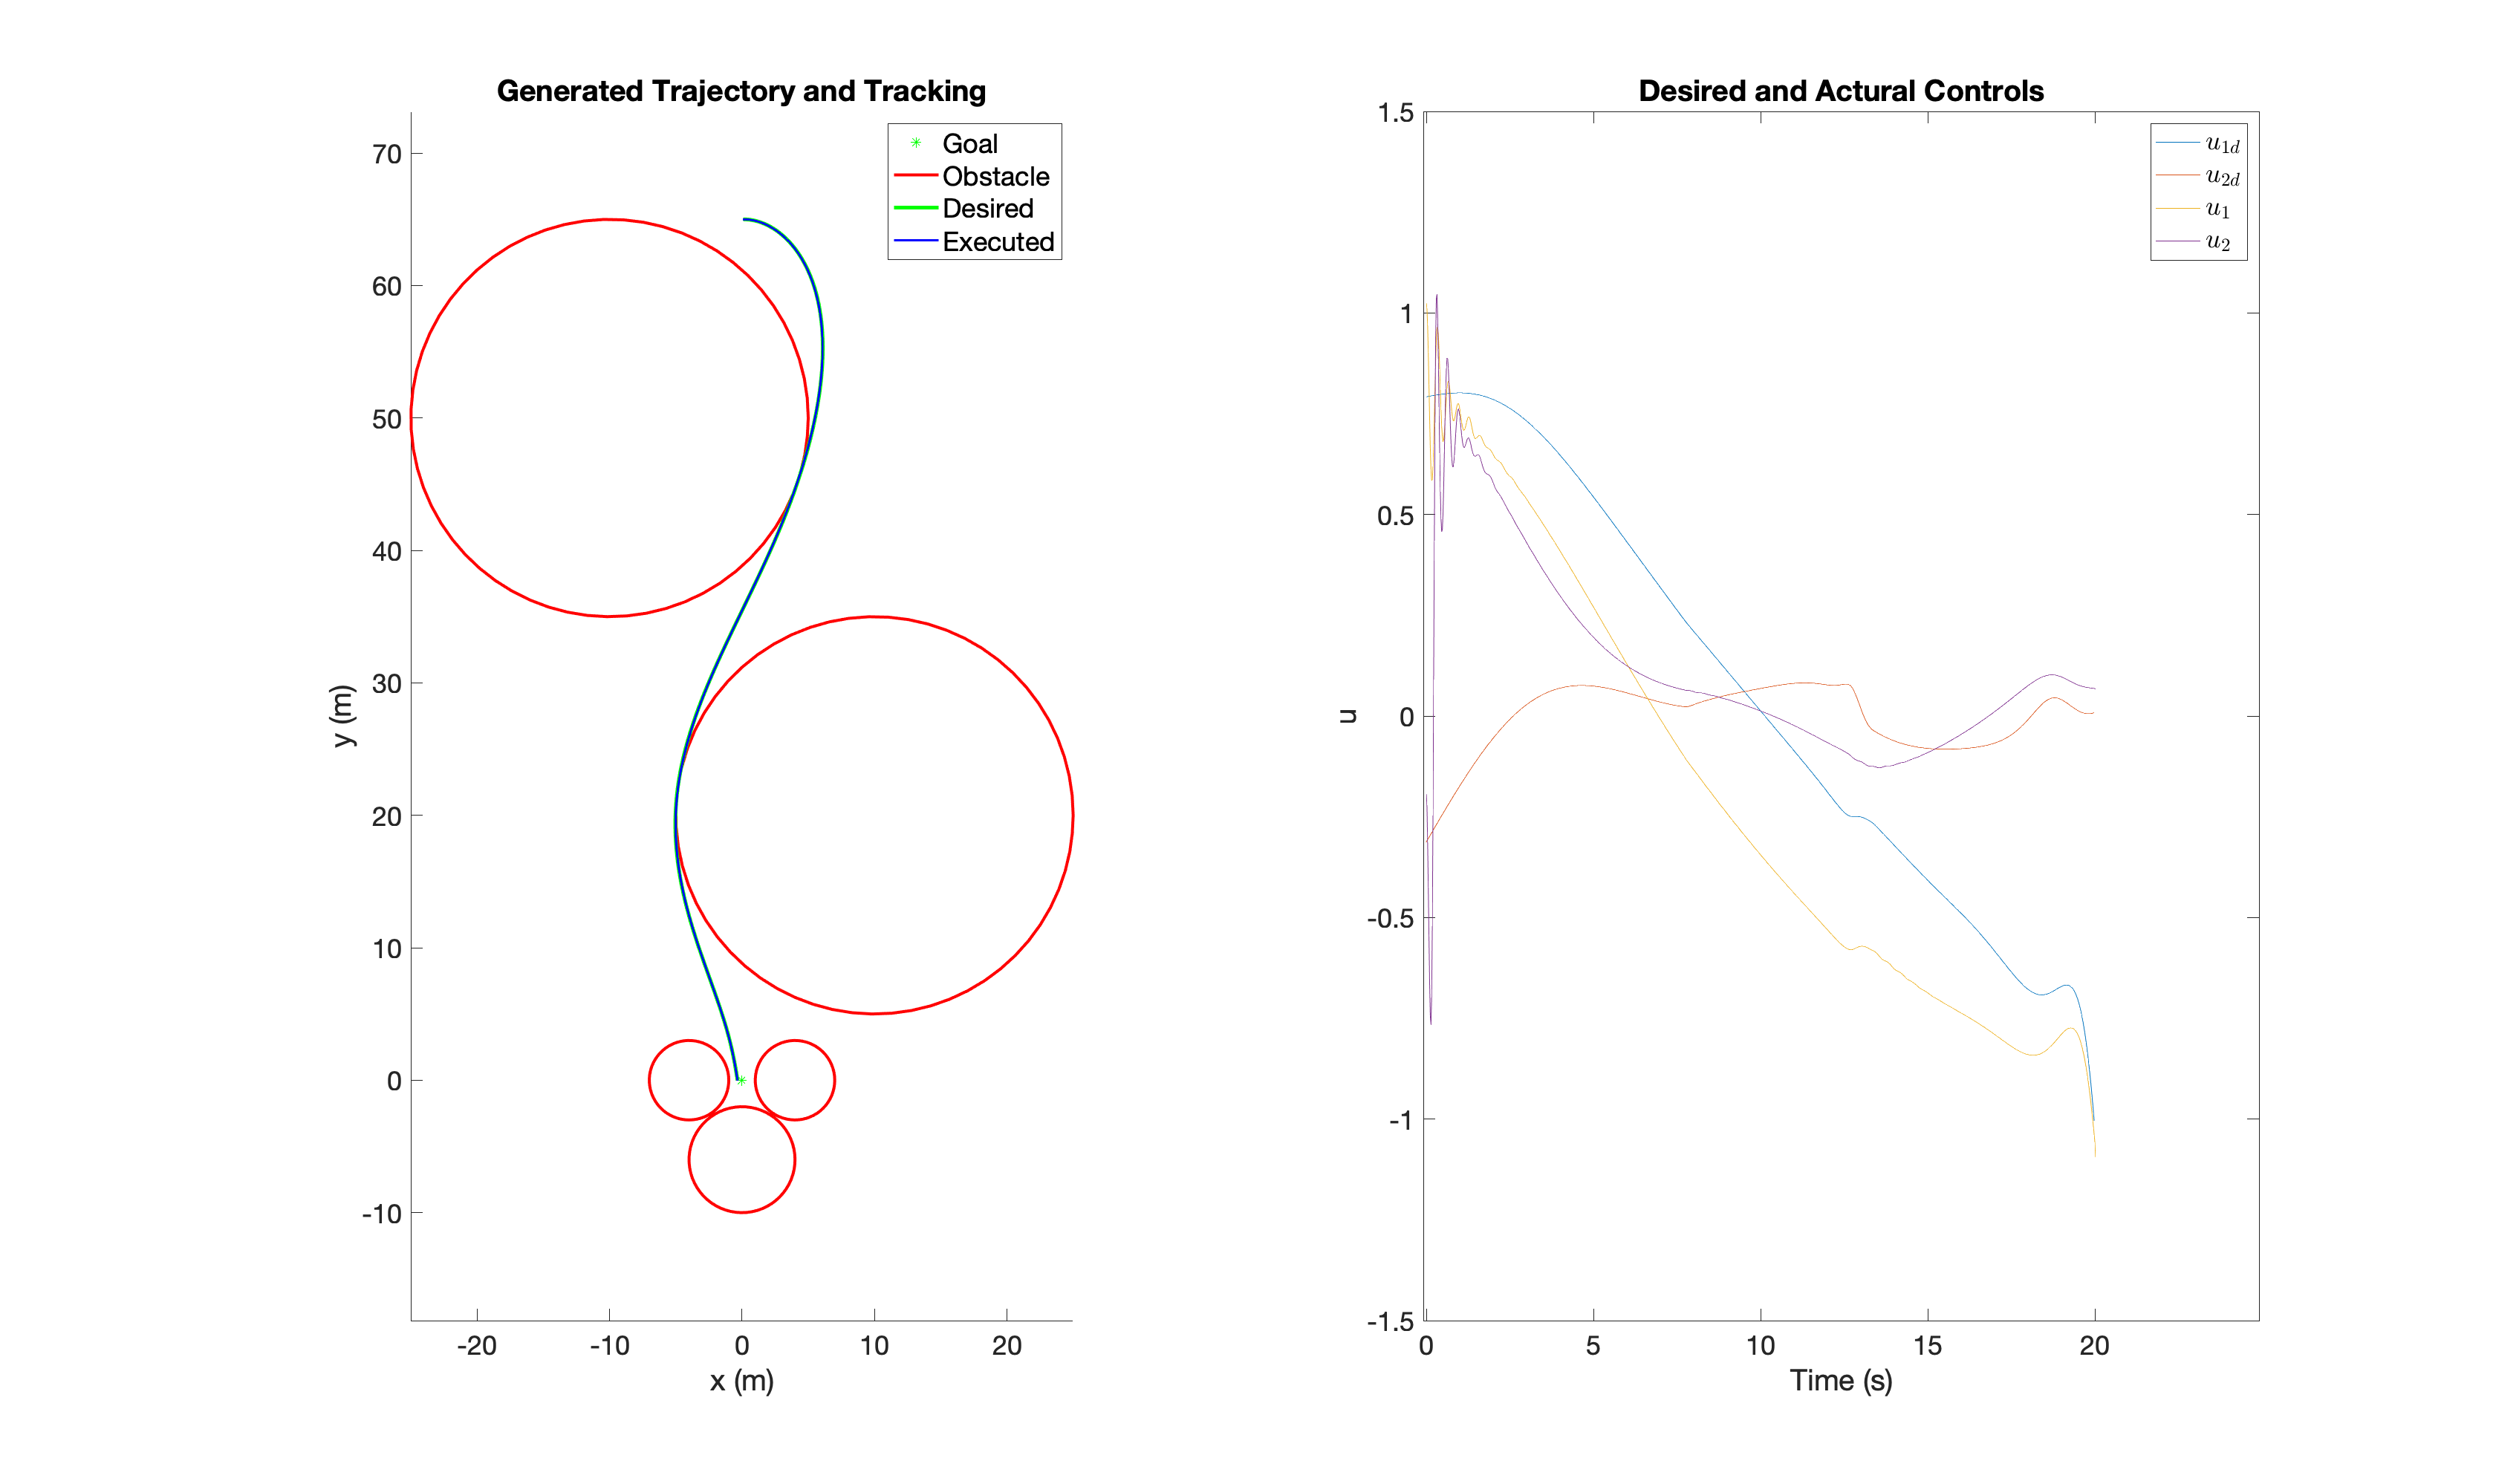
\includegraphics[width=\textwidth]{./figures/plot_and_controls.png}
    \caption{X Y plot of desired and executed trajectory and Controls plot}
    \label{fig:my_label}
\end{figure}

\begin{figure}[t]
    \centering
    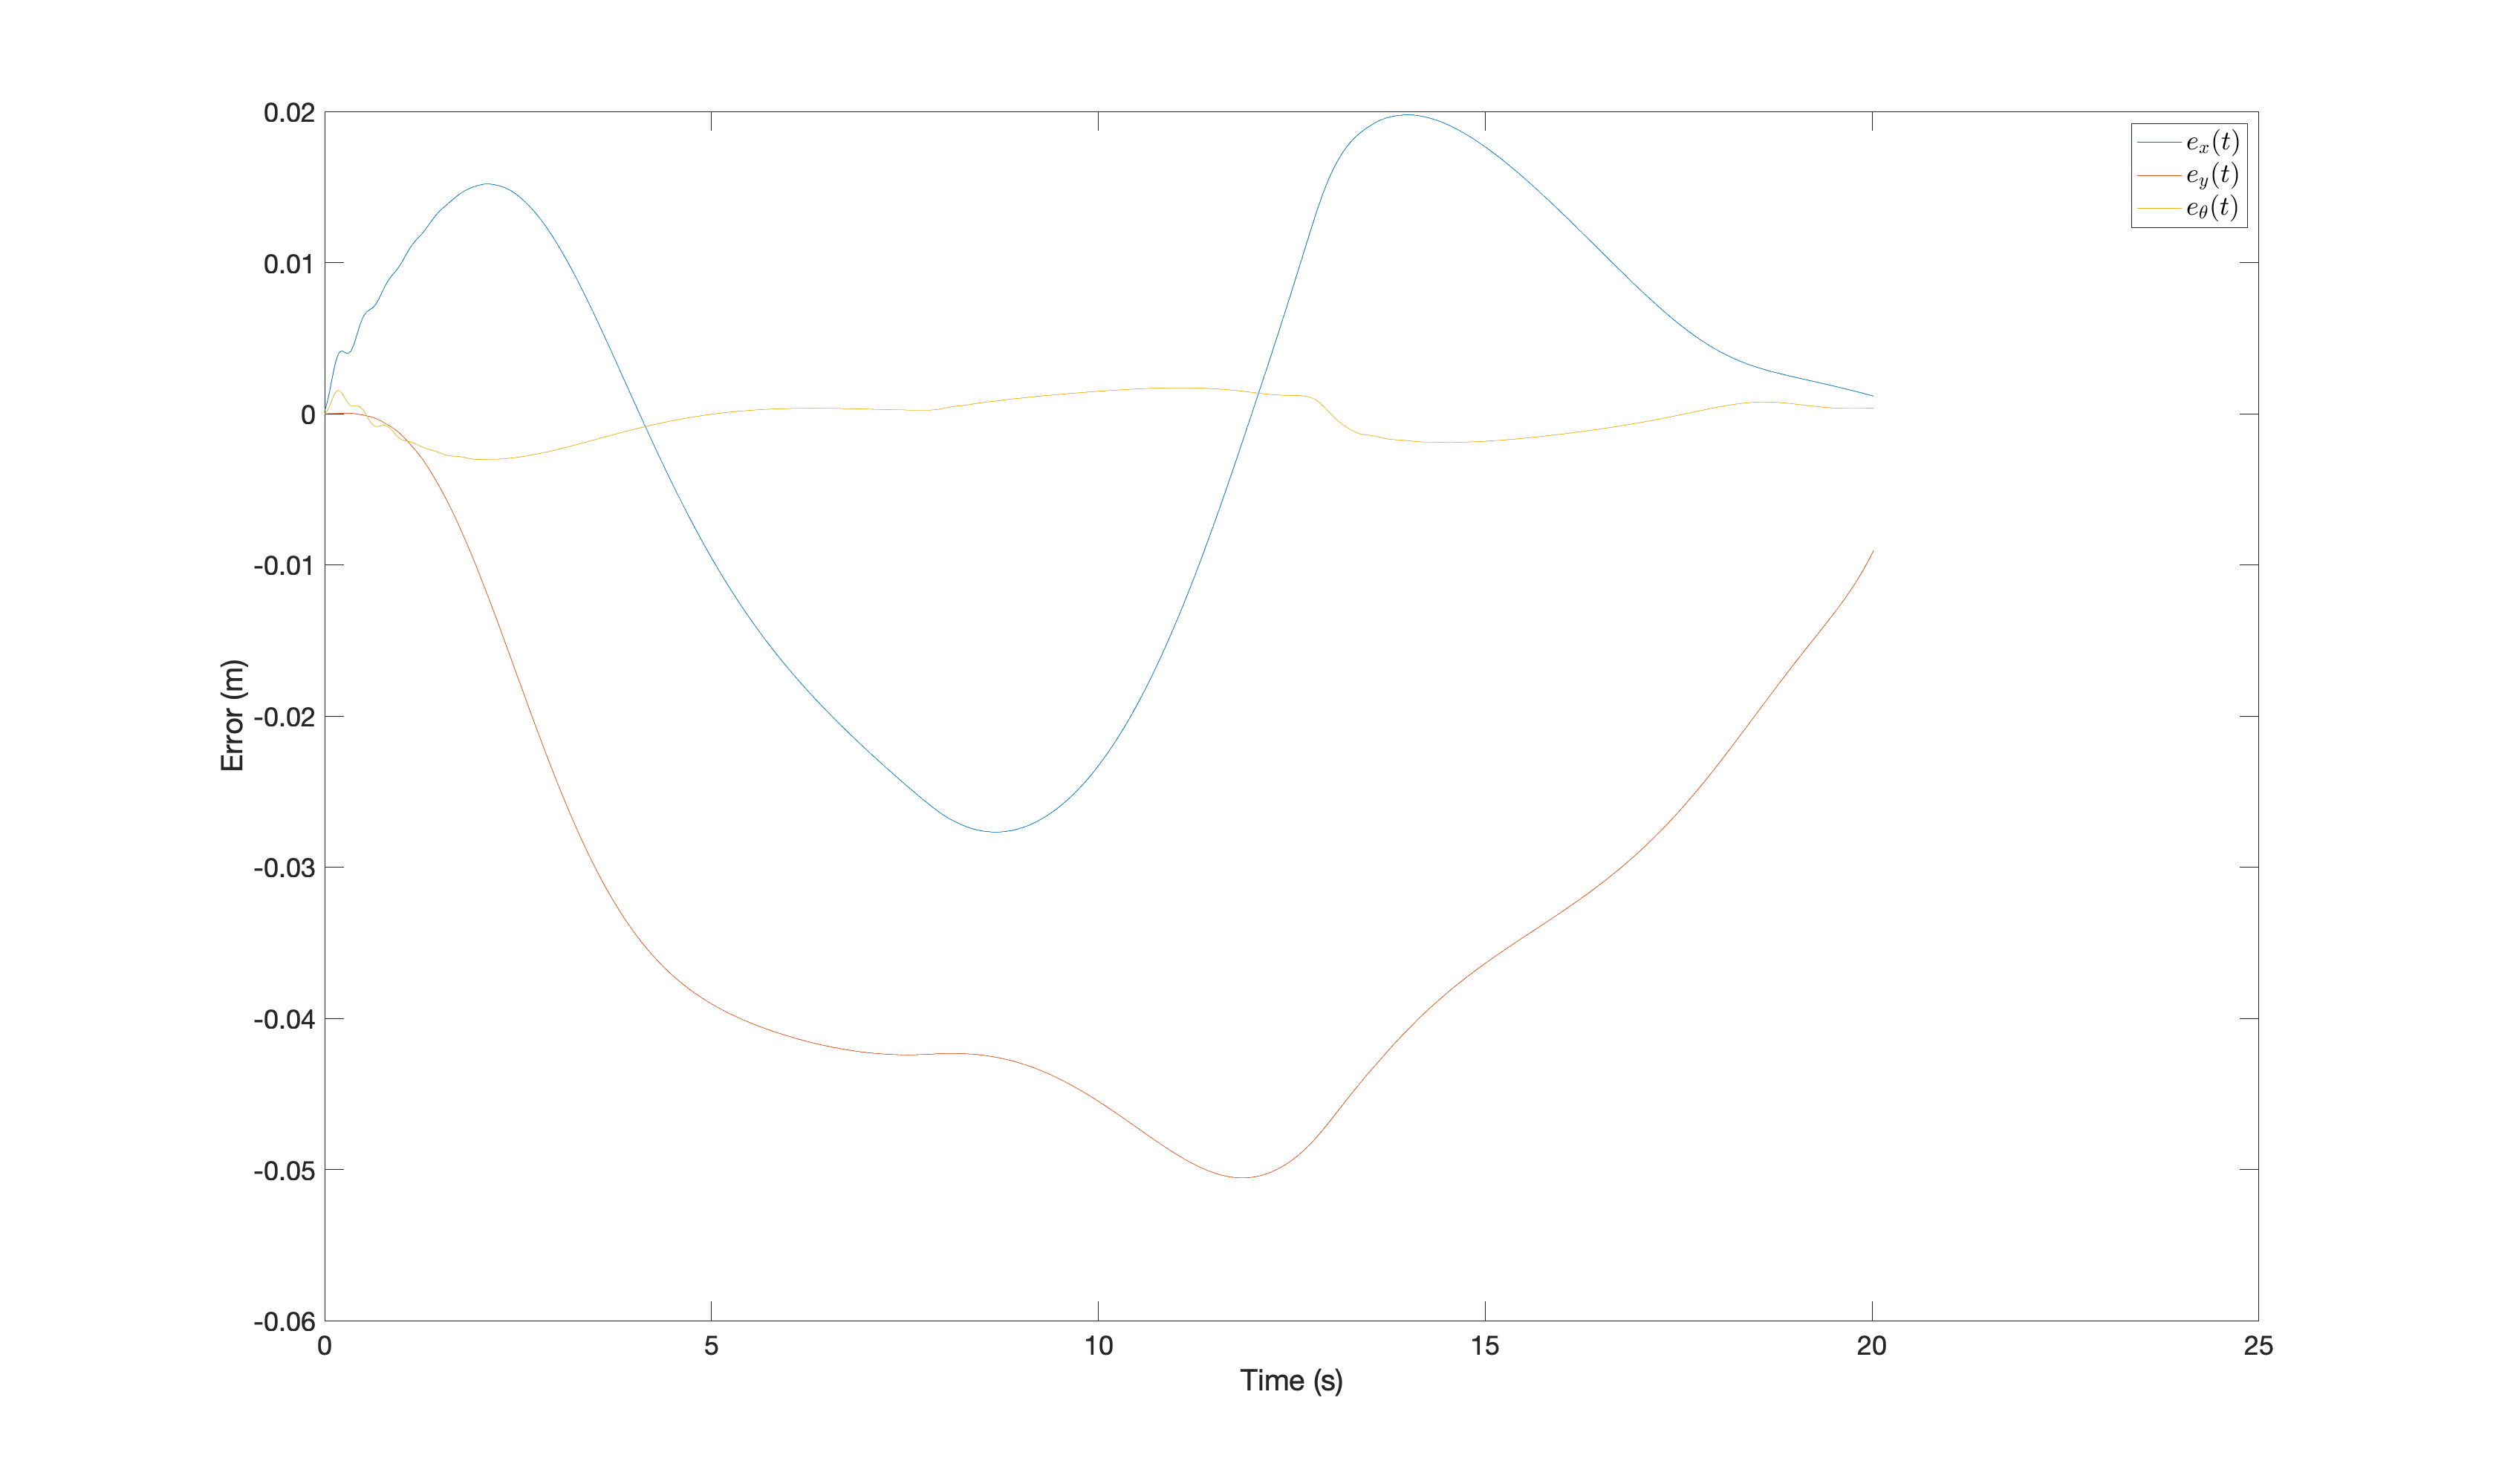
\includegraphics[width=\textwidth]{./figures/Error.png}
    \caption{Plot of errors over time}
    \label{fig:my_label}
\end{figure}
\end{document}
